%{{{Header
\documentclass[a4paper,10pt]{article}
\usepackage{anysize}
\marginsize{2cm}{2cm}{1cm}{1cm}
\usepackage{xltxtra}
\usepackage{graphicx}
\usepackage{color}
\usepackage{xgreek}
\usepackage{fancyvrb}
\usepackage{minted}
\usepackage{listings}
\usepackage{enumitem}
\usepackage{framed}
\usepackage{relsize}
\usepackage{float}
\setmainfont[Mapping=TeX-text]{DejaVu Serif}
%\documentclass[a4paper,12pt]{article}
\usepackage{xunicode}
\usepackage{pstricks}
\usepackage{pst-node}
\usepackage{pst-blur}
%}}}
\begin{document}

\def\thesection {\roman{section}: }
\def\thesubsection {\Roman{subsection}) }

\begin{titlepage}
\begin{center}

\noindent\begin{minipage}[b]{.55\textwidth}
\begin{Large}
\emph{Εθνικό Μετσόβιο Πολυτεχνείο\\
Σχολή ΗΜ\&ΜΥ\\
Προηγμένα Θέματα \\   Αρχιτεκτονικής Υπολογιστών\\
8\textsuperscript{ο} εξάμηνο, Ροή Υ\\
Ακαδημαϊκό Έτος: 2012\\}
\end{Large}
\end{minipage}%
\begin{minipage}[b]{.45\textwidth}
     \centering
     
\includegraphics[scale=0.8]{title/ntua_logo}
\end{minipage}

\vspace{5cm}
\begin{huge}
\underline{2\textsuperscript{η} Σειρά Ασκήσεων}
\end{huge}
\vfill

\begin{flushright}
\Large{Γερακάρης Βασίλης}\\
\large{<vgerak@gmail.com> }\\
\large{Α.Μ.: 03108092}\\
\end{flushright}
\vspace{1cm}

\large\today\\
\end{center}
\end{titlepage}



\section*{Εισαγωγή}

Στην άσκηση αυτή χρησιμοποιήσαμε ένα C++ Framework για την εξομοίωση
προβλεπτών αλμάτων,
όπως έχουν καταγραφεί από την εκτέλεση benchmarks της SPEC2000. Τα
trace files που μας δώθηκαν περιέχουν τις εντολές άλματος που πραγματοποιήθηκαν κατά την
εκτέλεση 100M εντολών.

%{{{ A1

\section*{Ν-bit predictors}


\subsection*{A.1}
Σε αυτό το τμήμα μελετήσαμε την απόδοση των Ν-bit predictors (1 εώς 7),
αξιολογώντας με βάση τα MPKI (Mispredictions Per
Thousand Instructions). Στο τμήμα αυτό είχαμε σταθερά BHT entries, ίσα με 16Κ.


\begin{figure}[H]
	\centering
	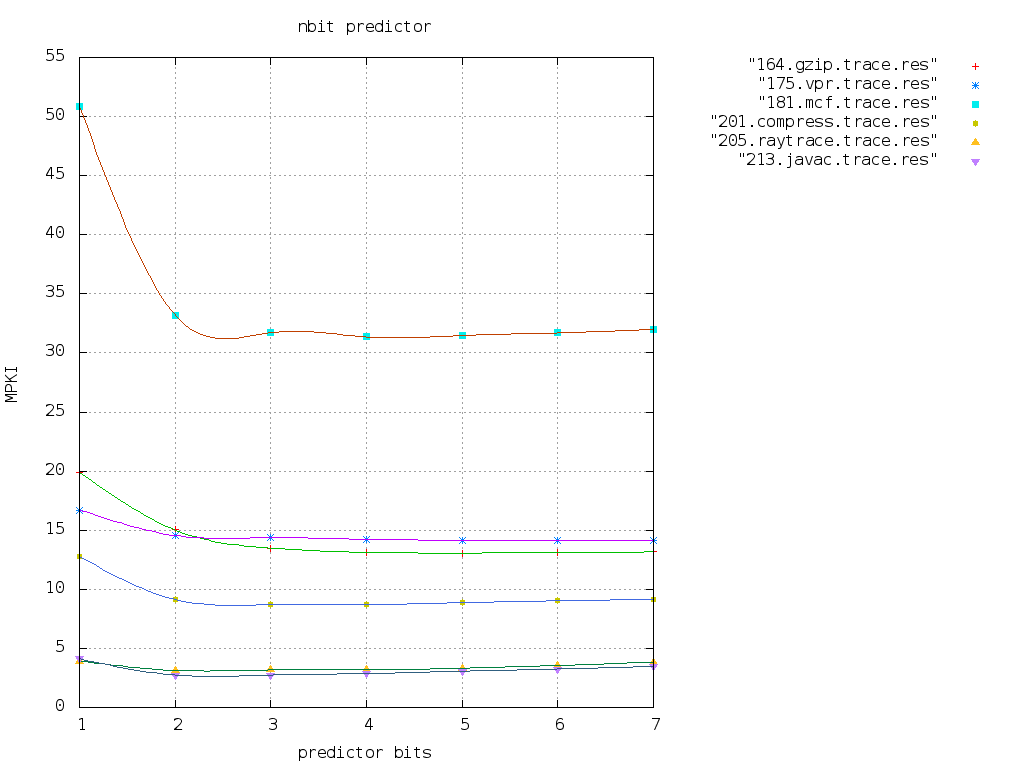
\includegraphics[width=0.8\textwidth]{../Results/part1/results_A1.png}
	\caption{1 to 7 - bit predictors}
\end{figure}


Όπως παρατηρούμε από το παραπάνω διάγραμμα, στα
περισσότερα benchmarks ο 4-bit predictor παρουσιάζει τη βέλτιστη επίδοση,
καθώς εκείνος εμφανίζει τα λιγότερα misspredictions, έχοντας ταυτόχρονα λίγες
απαιτήσεις από hardware.


%}}}

\pagebreak

%{{{ A2

\subsection*{A2}
Στο κομμάτι αυτό, μελετάμε τους \{1,2,4\}-bit predictors, αξιολογόντας πάλι με
βάση τα MPKI. Αυτή τη φορά, έχουμε σταθερό hardware και ίσο με 32Κ, και
μεταβάλλουμε το πλήθος των BHT entries.
\\

\begin{tabular}{c c c}
	HW & bits & BHT entries \\
	\hline
	\hline
	32K & 1 & 32K	\\
	\hline
	32K & 2 & 16K	\\
	\hline
	32K & 4 & 8K	\\
\end{tabular}

\begin{figure}[H]
	\centering
	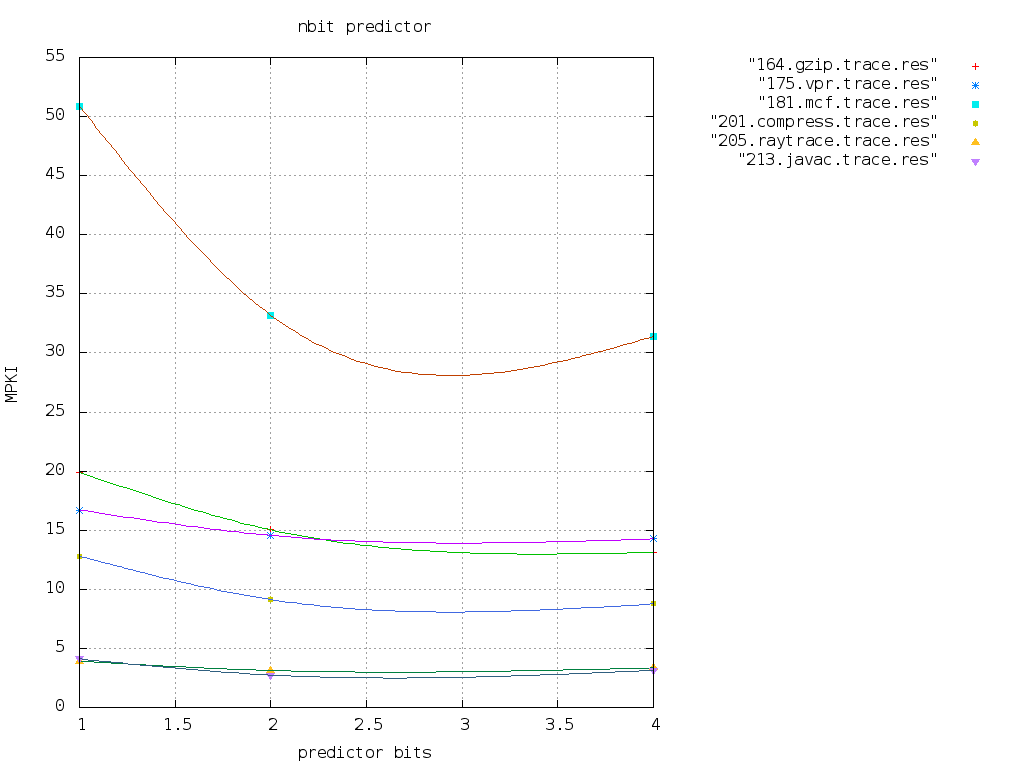
\includegraphics[width=0.8\textwidth]{../Results/part2/results_A2.png}
	\caption{1,2,4 - bit predictors}
\end{figure}

Παρατηρούμε πως ακόμα και στην περίπτωση που το hardware είναι σταθερό (32K),
καλύτερη απόδοση εμφανίζει ο 4 bit predictor.

%}}}
\pagebreak

%{{{ B1

\section*{BTB predictor}

\begin{tabular}{c c}
	btb\_lines & btb\_assoc \\
	\hline
	\hline
	512K & 1 \\
	\hline
	256K & 2 \\
	\hline
	128K & 4 \\
	\hline
	64K  & 8 \\

\end{tabular}

\begin{figure}[H]
	\centering
	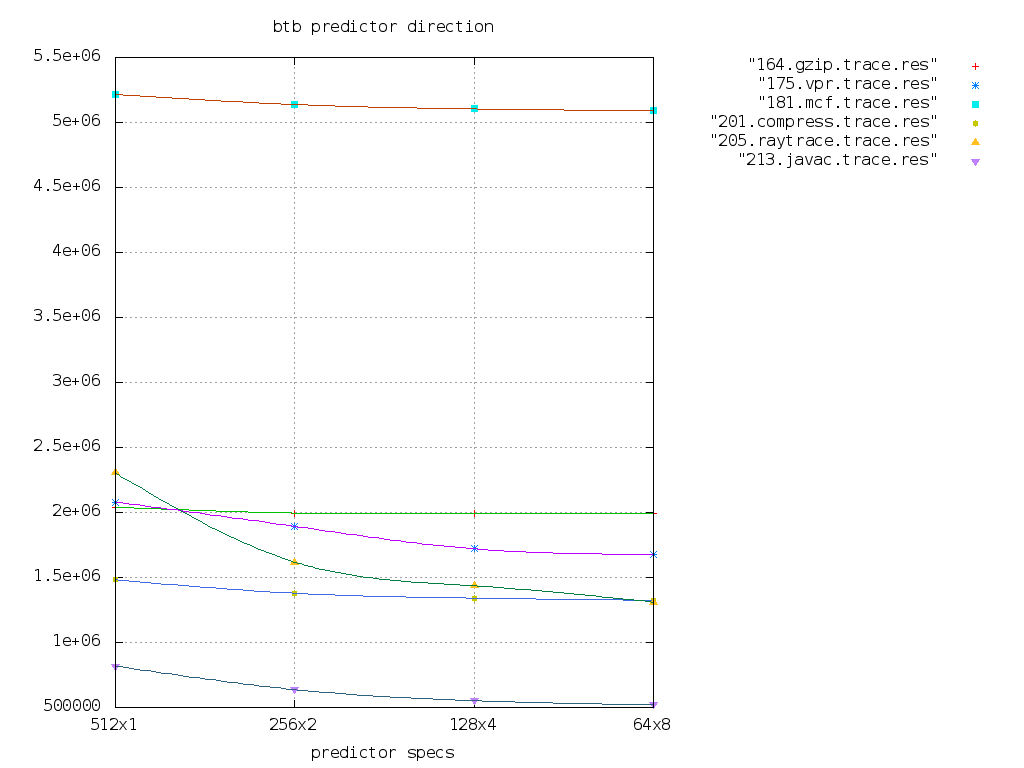
\includegraphics[width=0.8\textwidth]{../Results/part3/results_B1_direction.png}
	\caption{Direction misspredictions (direction MPKI)}
\end{figure}

\begin{figure}[H]
	\centering
	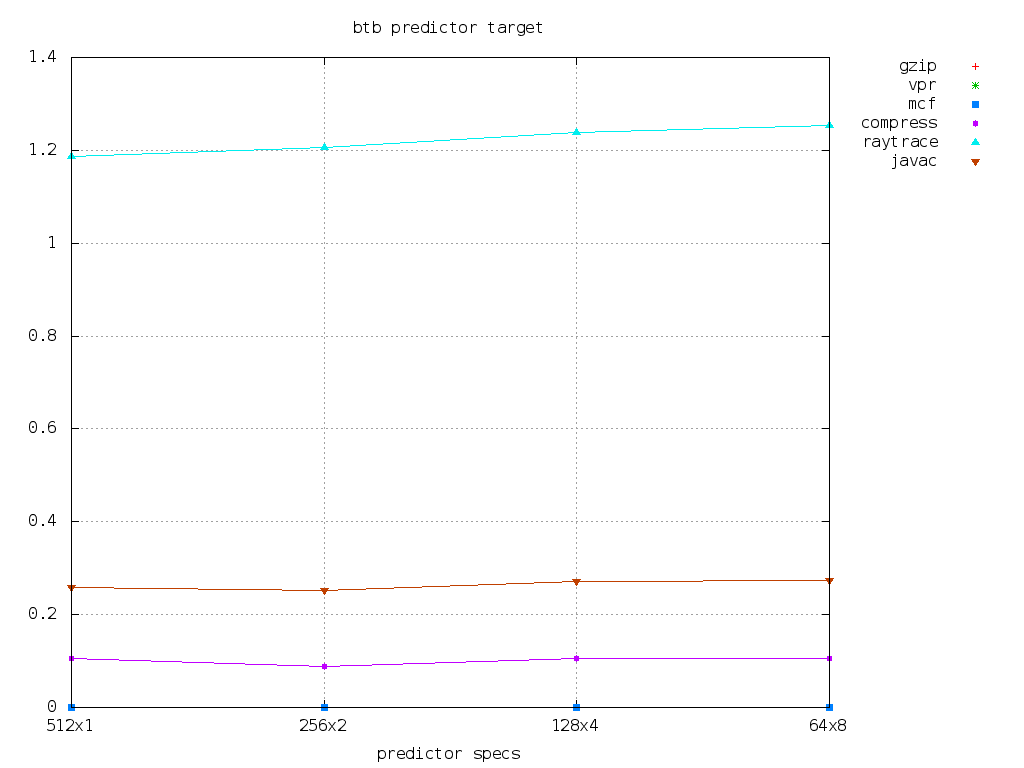
\includegraphics[width=0.8\textwidth]{../Results/part3/results_B1_target.png}
	\caption{Target Misspredictions (target MPKI)}
\end{figure}


Παρατηρούμε πως το target missprediction παραμένει σταθερό σχεδόν και είναι
συγκριτικά αμελητέο, σε αντίθεση
με το direction missprediction. Αυτό παρατηρούμε πως μειώνεται δραστικά στον
64x8 BTB predictor, οπότε επιλέγεται ως η επιθυμητή οργάνωση για τον BTB.

%}}}
%
%{{{ C1

\section*{C1. Σύγκριση διαφορετικών predictors}
\begin{figure}[H]
	\centering
	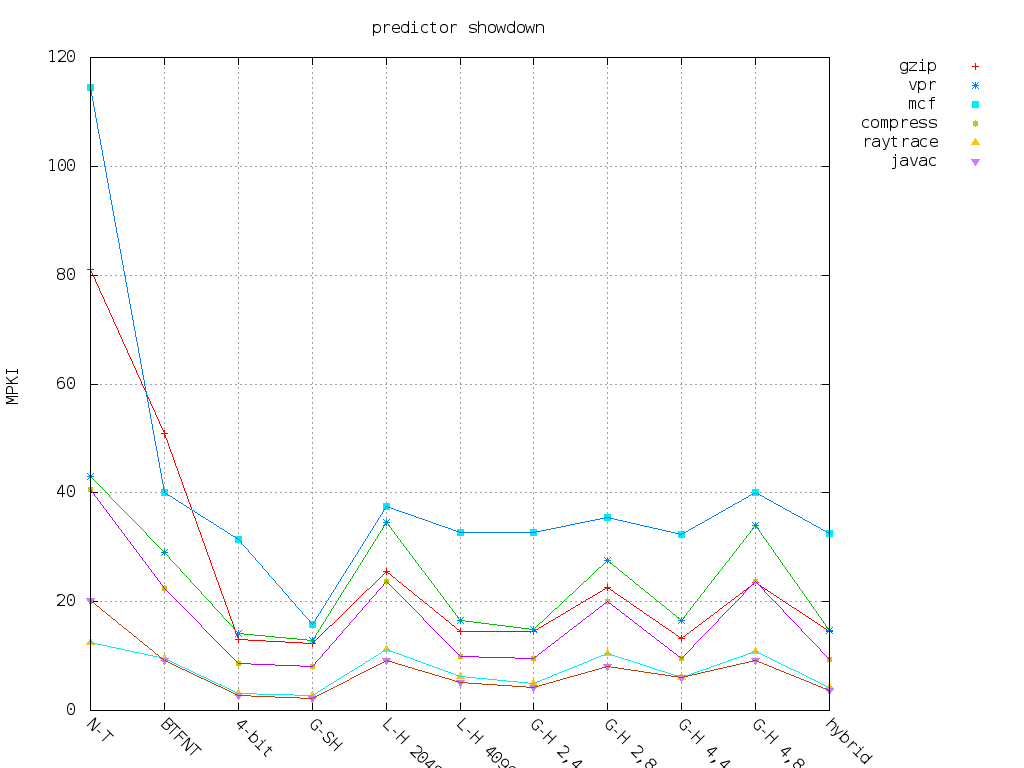
\includegraphics[width=0.8\textwidth]{../Results/part4/results_C1.png}
	\caption{Σύγκριση predictors}
\end{figure}


\section*{Source Code}
Ο πηγαίος κώδικας που χρησιμοποιήσαμε για τους predictors είναι ο ακόλουθος:

\subsection*{Static Not-Taken}
\inputminted[linenos,fontsize=\scriptsize,frame=leftline]{cpp}{files/ntaken.h}

\subsection*{Static Backward Taken Forward Not Taken}
\inputminted[linenos,fontsize=\scriptsize,frame=leftline]{cpp}{files/btfnt.h}

\subsection*{4-bit predictor}
\inputminted[linenos,fontsize=\scriptsize,frame=leftline]{cpp}{files/nbit_predictor.h}

\subsection*{gshare predictor}
\inputminted[linenos,fontsize=\scriptsize,frame=leftline]{cpp}{files/gshare_predictor.h}

\subsection*{Local-History two-level predictors}
\inputminted[linenos,fontsize=\scriptsize,frame=leftline]{cpp}{files/lhistory.h}

\subsection*{Global-History two-level predictors}
\inputminted[linenos,fontsize=\scriptsize,frame=leftline]{cpp}{files/ghistory.h}

\subsection*{Predict.cc}
\inputminted[linenos,fontsize=\scriptsize,frame=leftline]{cpp}{files/predict.cc}

\subsection*{Script για εκτέλεση benchmarks}
\inputminted[linenos,fontsize=\scriptsize,frame=leftline]{bash}{files/run.sh}


%}}}

\end{document}
